\chapter{Cronograma das atividades}\label{ape:cronograma}

Este apêndice apresenta o cronograma das atividades durante todo o desenvolvimento dessa pesquisa e das etapas que ainda
estão por vir. Cada atividade está numerada no cronograma e explicada em detalhe abaixo.

\begin{figure}[htb]
  \begin{center}
      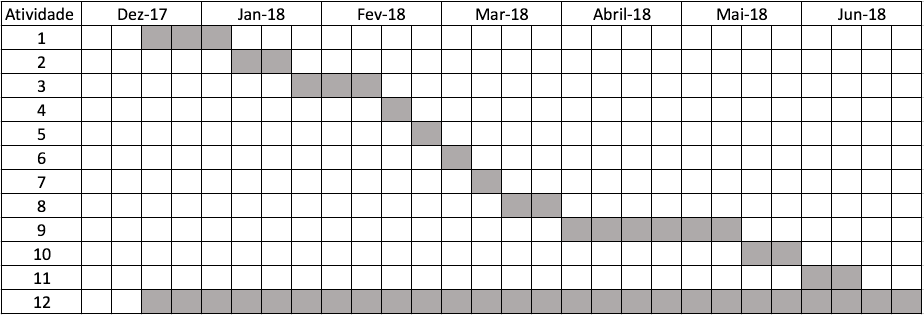
\includegraphics[scale=0.45]{./Figuras/cronograma.png}
  \end{center}
\end{figure}

\begin{enumerate}
\item Implementar a interface das recomendações
\item Analisar ferramentas para facilitar o cálculo da similaridade do perfil do usuário com os itens
\item Implementar os algoritmos de recomendação (tradicional e a proposta desse trabalho)
\item Melhorar a categorização (palavras-chave) dos materiais e Links de Apoio presentes no minicurso de algoritmos
\item Realizar testes para garantir a funcionalidade dos algoritmos de recomendação desenvolvidos
\item Produzir os intrumentos necessários para o experimento
\item Convidar alunos a participar do experimento
\item Realizar o experimento
\item Estudar e definir as técnicas de análise dos dados
\item Analisar os dados (resultados do experimento)
\item Escrever a dissertação
\end{enumerate}
